\section{Methode nach Stam}

\subsection{Motivation}

Die Methode zur approximativen Lösung der Navier-Stokes-Gleichungen, die im
Folgenden erklärt wird, wurde von \PimiddyName{Jos Stam} im Jahr 1999 entwickelt
und in dem Paper "`Stable Fluids"' vorgestellt \cite{Stam1999}. Das Verfahren
wurde speziell für die Computergrafik entwickelt, wobei auf einige
Besonderheiten eingegangen wurde:

\begin{enumerate}
\item
	Im Gegensatz zu wissenschaftlichen Simulationen ist man in der
	Computergrafik an einer Lösung interessiert, die in möglichst kurzen
	Abständen Ergebnisse produziert. Zum Beispiel möchte man die
	Strömungssimulation jedes Frame um einen Zeitschritt weiterbewegen. Um
	eine flüssige Simulation zu erhalten, ist die Laufzeit des
	Lösungsalgorithmus also auf 16 Millisekunden (für 60 Bilder pro Sekunde)
	bzw. 33 Millisekunden (für 30 Bilder pro Sekunde) beschränkt. Die
	Navier-Stokes-Gleichungen bilden als System von nichtlinearen
	Differentialgleichungen hier eine besondere Herausforderung.
\item
	Man ist außerdem nicht unbedingt an einer exakten Lösung interessiert.
	Will man z.B. Wasser oder Rauch simulieren reicht es, ein physikalisch
	annähernd korrektes Verhalten zu erzielen.
\item
	Bisherige Verfahren (wie z.B. die finiten Differenzen in
	\cite{Foster1997}) waren numerisch \emph{instabil} für große
	Zeitschritte. Dynamische Anwendungen wie Spiele oder Animationssoftware
	können allerdings keine minimiale Framerate garantieren, da sie mit
	verschiedenen Umgebungen und Hardwarekonfigurationen ausgeführt werden
	können.

	Als Ausweg muss man einen großen Zeitschritt (ein langes Frame) entweder
	ignorieren -- was die Simulation unrealistisch macht -- oder ihn in
	kleinere Zeitschritte unterteilen. Die Laufzeit des Verfahrens ist aber
	im Allgemeinen nicht von der Größe des Zeitschritts abhängig. Dies führt
	dazu, dass das nächste Frame erneut viel Rechenzeit benötigt und wieder
	entsprechend lang wird.

	Dieser Effekt ist nicht mehr aufzuhalten und die Simulation
	\PimiddyQuotes{explodiert}.
\item
	Bisherige Verfahren waren auf Hilfe des Designers angewiesen, um Teile
	der Simulation möglichst realistisch zu modellieren. Bestimmte natürlich
	vorkommende Turbulenzen mussten explizit in die Simulation eingegeben
	werden. Idealerweise sollte die Simulation allerdings von selber
	fortgeführt werden, der Designer sollte nur Rahmenbedingungen wie
	Hindernisse und globale Eigenschaften des Fluids (wie Dichte und
	Viskosität) vorgeben.
\end{enumerate}

\begin{figure}[ht]
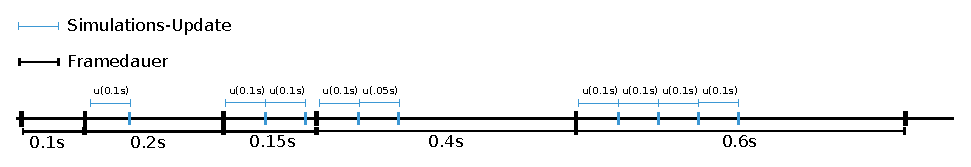
\includegraphics[width=12cm]{images/simulation_blowup}
\caption{Instabilität in Simulationen: Hier wird angenommen, die maximal zu simulierende Simulationsdauer sei $0.1s$. Längere Frames werden in mehreren Ticks berechnet, die aber konstant lange Laufzeit haben. Dies führt zu dauerhaft langen Frames, der Effekt potenziert sich.}
\end{figure}

Das Verfahren ist also auf Geschwindigkeit ausgelegt, basiert aber
nichtsdestotrotz auf den Navier-Stokes-Gleichungen und erzielt akkurate
Simulationsergebnisse. Anfängliche Schwachstellen des Verfahrens wie die zu
starke Dämpfung von Wirbeln wurden in weiteren Arbeiten ausgebessert
\cite{Foster}. Diese Verbesserungen sind teilweise auch in die Arbeit
eingeflossen.

Wegen der numerischen Stabilität und sehr guten Parallelisierbarkeit wird Stams
Verfahren bereits in einigen Spielen eingesetzt (siehe \cite{Crane2007},
\cite{Peschel2009}). Hier beschrieben wird eine leicht abgewandelte
Fassung, bei der andere Randbedingungen verwendet werden.

\subsection{Überblick über das Verfahren}

Die Fluidsimulation findet auf einem kollokierten Gitter statt.

Die Fluidsimulation findet auf einem diskreten, endlichen Gitter, also einer
Teilmenge von $\PimiddyGanz^n$ statt. Gegeben sei ein anfängliches Strömungsfeld
$\vec{u}$. In diesem Feld könnten z.B. alle Geschwindigkeitsvektoren auf eine
vorgegebene \PimiddyQuotes{Windrichtung} gesetzt sein. Gegeben sei außerdem ein
Zeitdelta $\Delta t$ (nicht zu verwechseln mit dem Laplaceoperator). Ziel ist
es, das Feld unter Zuhilfenahme der Navier-Stokes-Gleichungen einen diskreten
Zeitschritt weiter zu bewegen.

Die rechte Seite Impulsgleichung \eqref{navier_stokes_momentum_equation} besteht
aus mehreren Summanden:

\begin{equation}
\vec{g} +
\nu \PimiddyLaplace \vec{u} -
\vec{u} \PimiddyDiv \vec{u} -
\frac{
	1
}
{
	\rho
}
\PimiddyGrad p
\end{equation}

Jeder dieser Summanden stellt eine Operation dar, die
separat behandelt werden kann:

\begin{itemize}
\item
	Der Term $\vec{g}$ umfasst schlicht das Aufsummieren aller äußeren
	Kräfte, die auf das Fluid wirken. Hierzu gehört sowohl die Schwerkraft
	als auch der von außen eingeführte Wind.
\item
	Der Term
	\begin{equation}
	\nu \PimiddyLaplace \vec{u}
	\end{equation}
	stellt die viskose \PimiddyBegriff{Diffusion} dar. Selbst wenn keine
	Kräfte auf das Fluid wirken, bewegt es sich durch Diffusionsprozesse
	weiter, so wie Farbe auf einem Blatt Papier verläuft.

	Dieser Term kann in Stams Verfahren ignoriert werden, er entsteht
	ohnehin durch Genauigkeitsfehler während der Advektion (siehe unten). So
	kann Performance eingespart werden, denn die Lösung dieses Terms ist
	sehr aufwändig.
\item
	Der Term
	\begin{equation}
	\vec{u} \PimiddyDiv \vec{u}
	\end{equation}
	stellt die \PimiddyBegriff{Advektion} dar. Das Vektorfeld wird entlang
	seiner eigenen Strömungsrichtung weiterbewegt.
\item
	Der \emph{Druck} des Fluids wird in dem Term
	\begin{equation}
	\frac{1}{\rho} \PimiddyGrad p
	\end{equation}
	zusammengefasst. Er dient später dazu, die Randbedingungen und die
	Unkomprimierbarkeit zu erzwingen.
\item
	Wie bei Differentialgleichungen üblich, müssen wir noch die
	\emph{Randbedingungen} behandeln.
\end{itemize}

\begin{figure}[ht]
\includegraphics[width=10cm]{images/stam_loop}
\caption{Die Simulationsschleife ohne Projektion.}
\end{figure}

Für jeden Term wird im Folgenden ein Lösungsalgorithmus vorgestellt. Allerdings
garantiert keiner dieser Algorithmen, dass das Fluid nach Anwendung noch
unkomprimierbar ist. Die zweite Bedingung
\ref{navier_stokes_incompressibility_condition} kann also verletzt sein, und
unsere Simulation ist nicht mehr akkurat.

Gesucht ist ein Operator $\PimiddyProjection$, der ein Vektorfeld auf ein
quellenfreies Vektorfeld abbildet. Hierzu bedient man sich eines Ergebnisses aus
der Vektoranalysis, der \PimiddyBegriff{Helmholtz-Zerlegung} (auch
Helmholtz-Hodge-Theorem oder Ladyzhenskaya-Theorem genannt): Sei $\vec{u}$ ein
zweimal stetig differenzierbares Vektorfeld auf
einem beschränkten Definitionsbereich, dann lässt $\vec{u}$ sich zerlegen in ein
\emph{quellenfreies} Vektorfeld $\vec{w}$ und den \emph{Gradienten} eines
Skalarfeldes $p$:

\begin{equation}
\vec{u} = \vec{w} + \PimiddyGrad p
\end{equation}

Diese Gleichung wollen wir nach $\vec{w}$ auflösen und dieses Feld dann für die
weiteren Schritte verwenden. Dazu wenden wir die Divergenz auf die Gleichung an
und nutzen aus, dass der Operator linear ist:

\begin{equation}
\PimiddyDiv \vec{u} = \PimiddyLaplace p
\end{equation}

Dies ist eine sogenannte \PimiddyBegriff{Poissongleichung}, und ihre Lösung ist
ein Standardproblem in der Physik. Es wird später ein Verfahren vorgestellt, was
die obige Gleichung nach $p$ auflösen kann. Damit können wir dann durch
Umstellen und Bildung des Gradienten $\vec{w}$ bestimmen:

\begin{equation}
\vec{w} = u - \PimiddyGrad p
\end{equation}

Wir definieren jetzt

\begin{equation}
\PimiddyProjection \colon \PimiddyReell^n \to \PimiddyReell^n
\end{equation}

als die Funktion, die ein Vektorfeld auf den quellenfreien Anteil der
Helmholtz-Zerlegung abbildet (ein Vektorfeld also quellenfrei
\PimiddyQuotes{macht}). Führt man diesen nach der Advektion aus, erhält man eine
stabile Simulation.

\begin{figure}[ht]
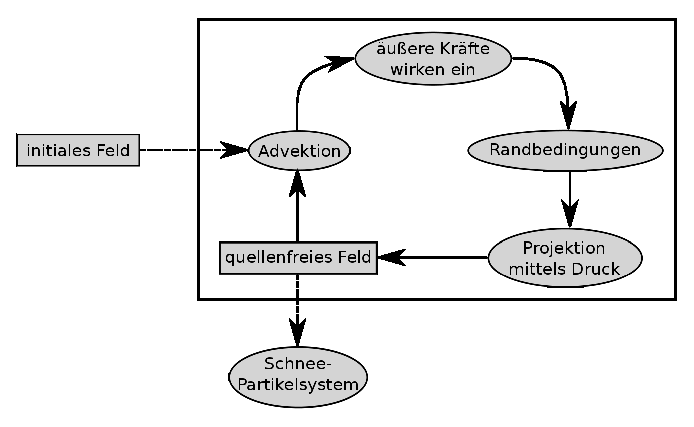
\includegraphics[width=10cm]{images/stam_loop_with_projection}
\caption{Die Simulationsschleife mit Projektion.}
\end{figure}

Definieren wir die einzelnen Schritte als Funktionen, ergibt sich im Pseudocode:

\begin{equation}
u^{t+\Delta t}
=
\PimiddyProjection(
	\PimiddyFormelText{advect}(
		\PimiddyFormelText{boundaries}(
			\PimiddyFormelText{externalforces}(
				u^t,
				\Delta t)),
		\Delta t))
\end{equation}

Im weiteren werden die Einzelschritte vorgestellt.

\subsection{Advektion}

Hier substanzielle Ableitung erklären? Oder schon früher bei den
Navier-Stokes-Gleichungen?

Wie bereits in der Erklärung der Navier-Stokes-Gleichungen angedeutet wird bei
der Advektion das Vektorfeld entlang seiner eigenen Geschwindigkeit
weiterbewegt. Im Folgenden gehen wir allgemeiner davon aus, dass eine beliebige
Größe $q(\vec{x},t)$ entlang des Vektorfelds $\vec{u}$ weiterbewegt werden soll,
also z.B. auch ein Temperaturwert oder die Rauchdichte.

Um diese Operation durchzuführen gibt es mehrere Ansätze. Der Intuitivste lässt
sich wie folgt beschreiben (\cite{Stam2003}):

Man stelle sich an jedem Gitterpunkt $\vec{i}=(i,j,k)$ ein Partikel mit
\PimiddyQuotes{Ladung} $q_{i,j,k}$. Durch das Vektorfeld würde das Partikel
um $\vec{u}_{i,j,k}$ verschoben und läge bei $\vec{p}=\vec{i}+\vec{u}_{i,j,k}$.
Somit läge es im Allgemeinen nicht mehr exakt auf einem Gitterpunkt, sondern
zwischen 8 Nachbarpunkten $n_i \in \PimiddyGanz^3, i \in \{1,\ldots,8\}$. Man bestimmt jetzt die
Distanz von $\vec{p}$ zu jedem der Nachbarpunkte:

\begin{equation}
d_i = \PimiddyNorm{2}{p - n_i}, i \in \{1,\ldots,8\}
\end{equation}

Diese $d_i$ dienen als Gewichtung, um die \PimiddyQuotes{Ladung} $q_{i,j,k}$
anteilig auf die Nachbarknoten aufzuteilen:

\begin{equation}
u_{n_i}' = u_{n_i}' + d_i \cdot q_{i,j,k}
\end{equation}

Dieses Verfahren ist intuitiv und einfach zu implementieren. Aber es ist
numerisch nicht stabil und führt zu Oszillationen (für eine genaue Betrachtung
sei auf die Literatur verwiesen).

Eine Alternative ist ein Ansatz mit finiten Differenzen wie in
\cite{Foster1997}. Dieser ist aber ebenfalls numerisch instabil.

Stam wählte einen anderen Ansatz, die sogenannte \emph{Methode der
Charakteristika}. Die Idee ist ähnlich zu der gerade vorgestellten, funktioniert
aber in die \PimiddyQuotes{umgekehrte Richtung}.

Wir betrachten wieder einen Gitterpunkt $\vec{i}=(i,j,k)$, nehmen diesmal aber
an, wir seien auf der Zeit-Achse im Punkt $t+\Delta t$, also bereits im nächsten
Zeitschritt. Das Partikel an Position $\vec{i}$ hat die Geschwindigkeit
$\vec{u}_{i,j,k}$. Rechnet man also auf der Zeitachse um $\Delta t$ zurück,
erhält man die \PimiddyQuotes{vorherige} Position des Partikels, nämlich
$\vec{i} - \Delta t \cdot \vec{u}_{i,j,k}$ \PimiddyFootnote{Hier wird nur ein
Schritt der Partikelflugbahn zurückverfolgt. Es gibt auch Methoden, die
mehrere Schritte verfolgen, diese sind aber aufwändig zu
implementieren.}. Es ergibt sich allerdings dasselbe
Problem wie bei dem vorher beschriebenen Ansatz: Diese Position liegt nicht
genau auf dem Gitter, sondern dazwischen.

Als Lösung interpolieren wir zwischen den 8 Nachbarwerten des verschobenen
Partikels und schreiben den entstehenden Wert in die Zelle $u'_{i,j,k}$. Dies
ist eine Operation, auf die Grafikkarten stark optimiert sind, und bei denen
traditionell Texturen hohe Performance erreichen können.

Natürlich kann es passieren, dass wir über den Rand des Simulationsbereiches
hinauslaufen. Hier können verschiedene Randbedingungen betrachtet werden.
Beispielsweise könnte man auf die gegenüberliegenden Seite des
Simulationsbereiches umbrechen (periodische Randbedingung), was in Stams Arbeit
getan wurde.

Alternativ kann man die Gitterpunkte, die am nächsten am Rand liegen, für die
Interpolation benutzen. Dies wurde in der Arbeit implementiert.

Weiterhin kann der zurückberechnete Vektor $\vec{i} - \Delta t u_{i,j,k}$ in
einem Hindernis landen. Man kann in diesem Fall einen Geschwindigkeitswert
von $(0,0,0)$ annehmen, was einem stationären Hindernis wie einem Gebäude
entspricht. Es ist aber auch möglich, ein weiteres Vektorfeld
$u_{\PimiddyFormelText{boundary}}$ zu verwalten, wo für jede Gitterzelle die
\emph{Geschwindigkeit} des dort vorhandenen Hindernisses notiert ist. Dies wurde
in \cite{Crane2007} umgesetzt. Für die Simulation in dieser Arbeit wurde von
unbeweglichen Hindernissen ausgegangen.

\PimiddyTodo{Hier noch Kommentar über die Stabilität (weil beim Interpolieren ja
	nichts \PimiddyQuotes{summiert} wird und so nichts größeres als das bisher dagewesene
	rauskommen kann. Außerdem steht in \cite{Foster}, dass man maximal 5
	Gridzellen weitergehen darf ohne zu viel Dissipation zu haben}

\subsection{Projektion}

\subsubsection{Lösung des Poissonproblems}

Um das Vektorfeld quellenfrei zu machen, muss folgende
\PimiddyBegriff{Poissongleichung} nach $p$ gelöst werden:

\begin{equation}
\PimiddyLaplace{p} = x
\end{equation}

wobei $x$ ein Skalarfeld ist. Es existieren zahllose Lösungsverfahren für so
eine Gleichung. Bei der Auswahl des Verfahrens muss beachtet werden, welches
sich gut auf der Grafikkarte umsetzen lässt. Hier haben sich mehrere sogenannte
\PimiddyBegriff{Iterationsverfahren} als günstig herausgestellt. Verfahren
dieser Art beginnen mit einer initialen Lösung (z.B. schlicht $p=0$) und nähern
sich dann in jedem Iterationsschritt weiter der eigentlichen Lösung an.

Betrachtet man große Felder, bieten sich \PimiddyBegriff{Mehrgitterverfahren}
an. Diese wurde bereits erfolgreich auf GPUs angewendet (siehe \cite{Bolz2002}),
sind allerdings untrivial zu implementieren, da intern ein zweites
Iterationsverfahren benötigt wird (der sogenannte Restriktionsoperator).

Simplere Iterationsverfahren sind SOR (umgesetzt in \cite{Saltvik2006}),
Gauss-Seidel-Re"-la"-xa"-ti"-on (umgesetzt in \cite{Stam2003}) und das
Jacobiverfahren (umgesetzt in \cite{Crane2007}, \cite{Harris2008},
\cite{Peschel2009}). Letzteres ist besonders einfach zu
implementieren und gleichzeitig hervorragend für die GPU geeignet.

\subsubsection{Das Jacobiverfahren}

Um das Jacobi-Verfahren zu veranschaulichen, betrachten wir das eindimensionale
Problem. Wir betrachten also kein diskretes 3D-Gitter, sondern eine Teilmenge
der ganzen Zahlen. Für die exakte Lösung $p$ des Poissonproblems muss an jeder
Stelle $p_i$ gelten (Randbedingungen werden später behandelt):

\begin{equation}
\label{stam_jacobi_onedimensional}
\frac{
	p_{i+1} -
	2 \cdot p_{i} +
	p_{i-1}
}
{
	2
}
=
x_i
\end{equation}

Angenommen wir hätten eine Anfangslösung $p^0$, z.B.
$p^0 = 0$. Dann können wir eine neue Lösung bestimmen,
indem wir \autoref{stam_jacobi_onedimensional} nach $p_i$ auflösen und dabei die
Nachbarwerte aus $p^0$ als Näherungen für die Nachbarn
in der exakten Lösung nehmen:

\begin{equation}
\label{stam_jacobi_onedimensional_iterative_solution}
p_i^1
=
\frac{
	x_i + p_{j+1}^{0} + p_{j-1}^{0}
}
{
	2
}
\end{equation}

Im nächsten Iterationsschritt berechnet man dann $p_i^2$ mit Hilfe von $p_i^1$,
usw., bis man nahe genug an die exakte Lösung herangekommen ist. In der Praxis
sind mindestens 20 Iterationen nötig, da das Verfahren sehr langsam konvergiert.

Eine leichte Konvergenzverbesserung erreicht man, indem man die rechte Seite von
\autoref{stam_jacobi_onedimensional_iterative_solution} nicht direkt als neue
Lösung nimmt, sondern zwischen der bisherigen Lösung und der neue Lösung mit
einem Gewichtungsfaktor $\omega$ interpoliert:

\begin{align}
\overline{p}_i^{n+1}
&=
\frac{
	x_i + p_{j+1}^{n} + p_{j-1}^{n}
}
{
	2
} \\
p_i^{n+1}
&=
(1-\omega) \cdot p_i^n + \omega \cdot \overline{p}_i^{n+1}
\end{align}

Dieses Verfahren wird \PimiddyBegriff{gewichtete Jacobi-Iteration} genannt. In
der Praxis hat sich ein Faktor von $\omega=\frac{2}{3}$ als günstig erwiesen.

\subsubsection{Randbedingungen}

Auch beim Druck müssen Randbedingungen betrachtet werden. Dies betrifft wiederum
den Rand der Simulation sowie Hinderniszellen.

Der Rand der Simulation soll so geartet sein, als wäre die Simulation an den
Seiten \PimiddyQuotes{offen}. Das Fluid soll am Simulationsrand nicht abprallen,
sondern sich dorthin weiter ausbreiten (outflow boundary conditions
\PimiddyTodo{verifizieren und übersetzen}). Um dies anzunähern verändern wir vor
dem Projektionsschritt das Geschwindigkeitsfeld so, dass die
Geschwindigkeitswerte am Rand denen \PimiddyQuotes{neben dem Rand} entsprechen.
So entsteht bei der Bildung des Drucks kein Unterschied zu den Nachbarzellen und
bei der Gradientbildung im nächsten Schritt ergibt sich $0$.

Für Hindernisse im Simulationsbereich wollen wir sogenannte
\PimiddyBegriff{free-slip}-Randbedingungen umsetzen. Wie der Name andeutet
erzwingen diese Randbedingungen, dass sich das Fluid (tangential) entlang des
Hindernisses bewegen kann aber nicht in das Hindernis hineinfließen darf.
Ist $\vec{n}$ die Normale an einem Punkt des Hindernisses und
$\vec{u}_{\PimiddyFormelText{Hindernis}}$ die Geschwindigkeit des Hindernisses,
dann muss im Geschwindigkeitsfeld des Fluids gelten:

\begin{equation}
\vec{u} \cdot \vec{n} = \vec{u}_{\PimiddyFormelText{Hindernis}} \cdot \vec{n}
\end{equation}

Da wir im weiteren $\vec{u}_{\PimiddyFormelText{Hindernis}}=0$ annehmen gilt:

\begin{equation}
\vec{u} \cdot \vec{n} = 0
\end{equation}

Ohne Herleitung stellen wir fest, dass sich dies sehr einfach in den
Jacobi-Algorithmus integrieren lässt. Wir testen für jede Nachbarzelle der
aktuellen Zelle, ob diese von einem Hindernis belegt ist. Ist dem so, ersetzen
wir den Druckwert durch den der aktuellen Zelle. Wir ignorieren also Nachbarn,
die von Hindernissen belegt sind.

Da der Jacobi-Algorithmus die Projektionsgleichung nur annähernd löst,
erzwingen wir am Ende die Randbedingungen für die Voxel, die an Hindernisse
angrenzen, explizit.

\subsection{Äußere Kräfte}

\subsubsection{Gravitation}

Zu den äußeren Kräften gehört zu allererst die \emph{Gravitation}. Diese lässt
sich sehr einfach ausdrücken:

\begin{equation}
F_g = \Delta t (0,-9.81,0)
\end{equation}

\subsubsection{Auftrieb}

\PimiddyTodo{Auftrieb allgemein und konkret mit Buissnesq erklären}

\subsubsection{Wirbelstärkenerhaltung}

\PimiddyTodo{Vorticity Confinement erklären.}
